\documentclass[runningheads]{llncs}

\usepackage[T1]{fontenc}
\usepackage{graphicx}
\usepackage{array}
\usepackage{booktabs}
\usepackage{tabularx}
\usepackage{todonotes}
\usepackage{amsmath}
\usepackage{paralist}
\usepackage{url}

% for problem descriptions
\newenvironment{problemdescription}
  {\begin{list}{}{\setlength{\leftmargin}{1cm}\setlength{\rightmargin}{1cm}}\item[]}
  {\end{list}}

% for text in math mode
\newcommand{\mt}[1]{\mathit{#1}}

\begin{document}

\title{Business Process Optimization}

\author{Remco Dijkman\inst{1} \and
Arik Senderovich\inst{2}}

\institute{Eindhoven University of Technology, The Netherlands\\
\email{r.m.dijkman@tue.nl}\\
\and
York University, Toronto, Canada\\
\email{sariks@yorku.ca}}

\maketitle

\begin{abstract}
Business Process Optimization (BPO) focuses on making optimal decisions during both the redesign and execution of business processes. These decisions include determining which resources to assign to specific tasks, how many resources to schedule at various times, when to admit or schedule particular cases, and how to route cases through alternative paths.
Moreover, the decisions must strike a balance between competing objectives, such as minimizing cost, reducing processing time, and enhancing customer satisfaction, while adhering to resource availability, deadlines, and budget limitations. The complexity of business process optimization lies in uncertainty in the arrivals of new cases, the duration of activity execution, and the paths that cases will take through the organization.
This paper provides a structured introduction to BPO by (i) classifying common decision-making problem types and relating them to operational, tactical, and strategic variants, (ii) presenting a framework of recurring components in solution approaches, (iii) defining a language for describing BPO problems precisely, and (iv) surveying representative problem--solution pairs to illustrate how these elements connect.
\end{abstract}


\section{Introduction}

Business Process Optimization (BPO) focuses on improving the efficiency and effectiveness of operational decision-making within business processes. This involves formulating and solving optimization problems that guide these decisions. Figure~\ref{fig:process} shows an illustrative example of a business process in which various BPO decisions may need to be taken. The process shows a banking process, modeled in BPMN (see~\cite{OMG_BPMN_2_0_2}), in which applications arrive at a rate of two per hour that is exponentially distributed. 

When an application arrives, an appointment needs to be planned for the customer who made the application. This is the first decision that needs to be made. Once the appointment is planned, the customer will arrive at the planned time of the appointment. Subsequently, a decision - modeled as an XOR-split - must be made on the type of application: whether it is considered a complex application or a simple application. Complex applications will be handled by a senior risk manager and simple applications will be handled by a junior risk manager. As the model shows, after the risk assessment the application either continues by drafting a proposal for the customer or the advice needs to be redone. Overall, there is a 20\% chance that the advice needs to be redone. However, one could imagine that this probability is higher when a simple advice is given as this may not take all the subtleties of the application into account. This does not mean that it is wise to process all applications as complex applications, because complex applications take longer to process and require senior rather than junior employees, who can also be expected to be more expensive. Consequently, deciding on whether an application should be processed as a simple or a complex application is a difficult decision that requires making a trade-off between the amount of time it will take to process the application, the cost of the personnel involved in processing the application, and the likelihood that the advice step will need to be redone - which in itself has an impact on time and cost as well as customer satisfaction as customers will probably not like it when their application must be revisited.

\begin{figure}[t!]
    \centering
    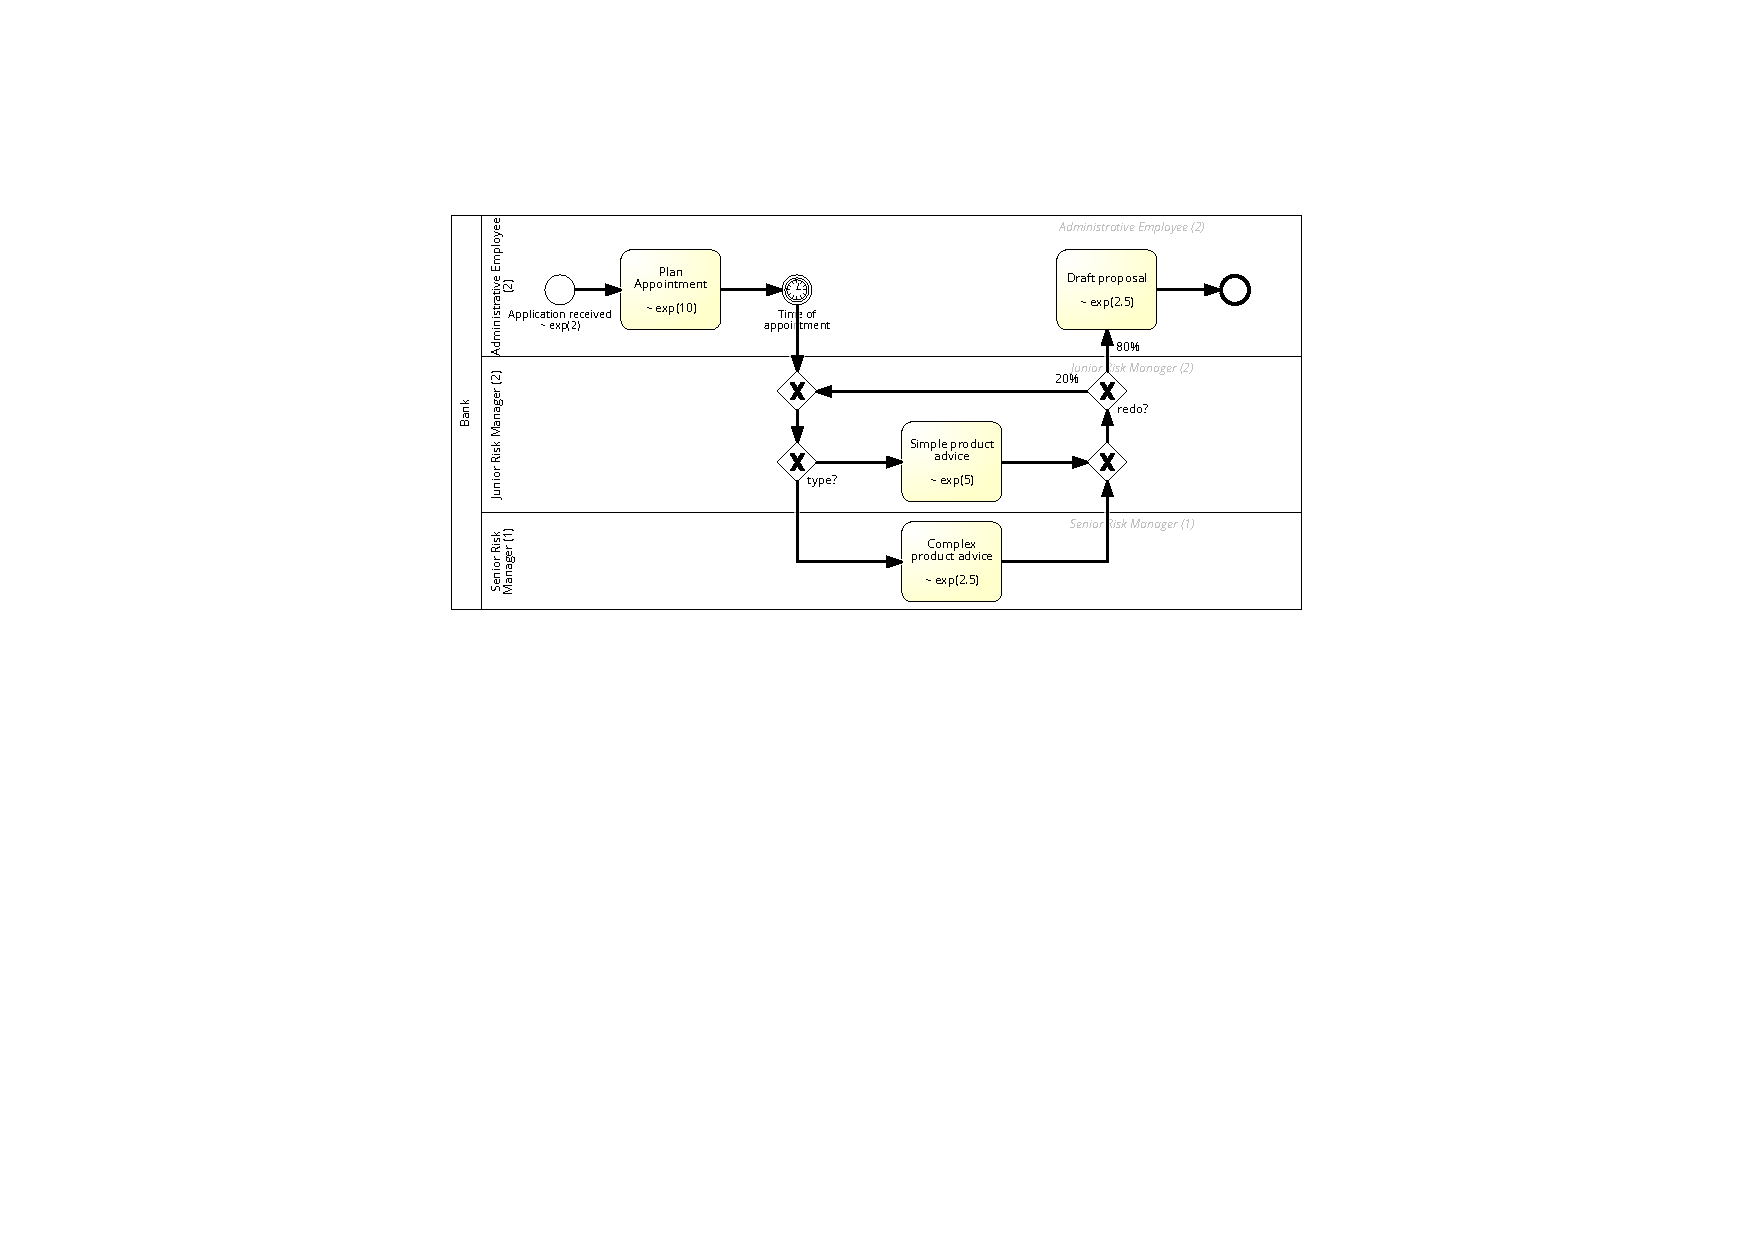
\includegraphics[width=0.9\linewidth]{figs/process.pdf}
    \vspace{-1em}
    \caption{A process with various BPO decisions.}
    \label{fig:process}
\end{figure}

This example illustrates two different types of BPO decision-making, but more exist. Different types of algorithms to solve these problems exist as well. For example, heuristic rules can be defined to take a decision on whether an application should be processed as a simple application or a complex application. Conversely, appointments can be scheduled once per week, for applications that arrived that week, by solving a complex Mixed Integer Linear Program (MILP).
Against this background, this paper presents an overview of different types of BPO decision making problems that have been discussed in the literature. It also presents an overview of the different types of solutions that have been used. 

These different types of solutions typically have similar components, which are organized in a framework.
Specifically, Section~\ref{sec:problems} introduces different types of BPO decision-making problems. Section~\ref{sec:framework} presents a framework comprising various components for solution approaches. Section~\ref{sec:problemdescription} defines a language for describing business process optimization problems, while Section~\ref{sec:solutionapproaches} outlines four typical solution approaches. Section~\ref{sec:survey} provides an overview of BPO problems and solution approaches covered in this paper, and Section~\ref{sec:conclusion} concludes the paper.

\section{BPO Decision-making Problems}\label{sec:problems}

This section presents and classifies different types of BPO decision-making problems, illustrating them with BPMN models. It serves as an inspiration for identifying and solving such problems in one's own organization, but does not claim to be a complete overview of possible problems. Still other problems can probably be envisioned and we encourage the reader to look out for these problems and research methods for solving them as well.

\subsection{Task Prioritization and Resource Allocation}
\begin{figure}[t!]
    \centering
    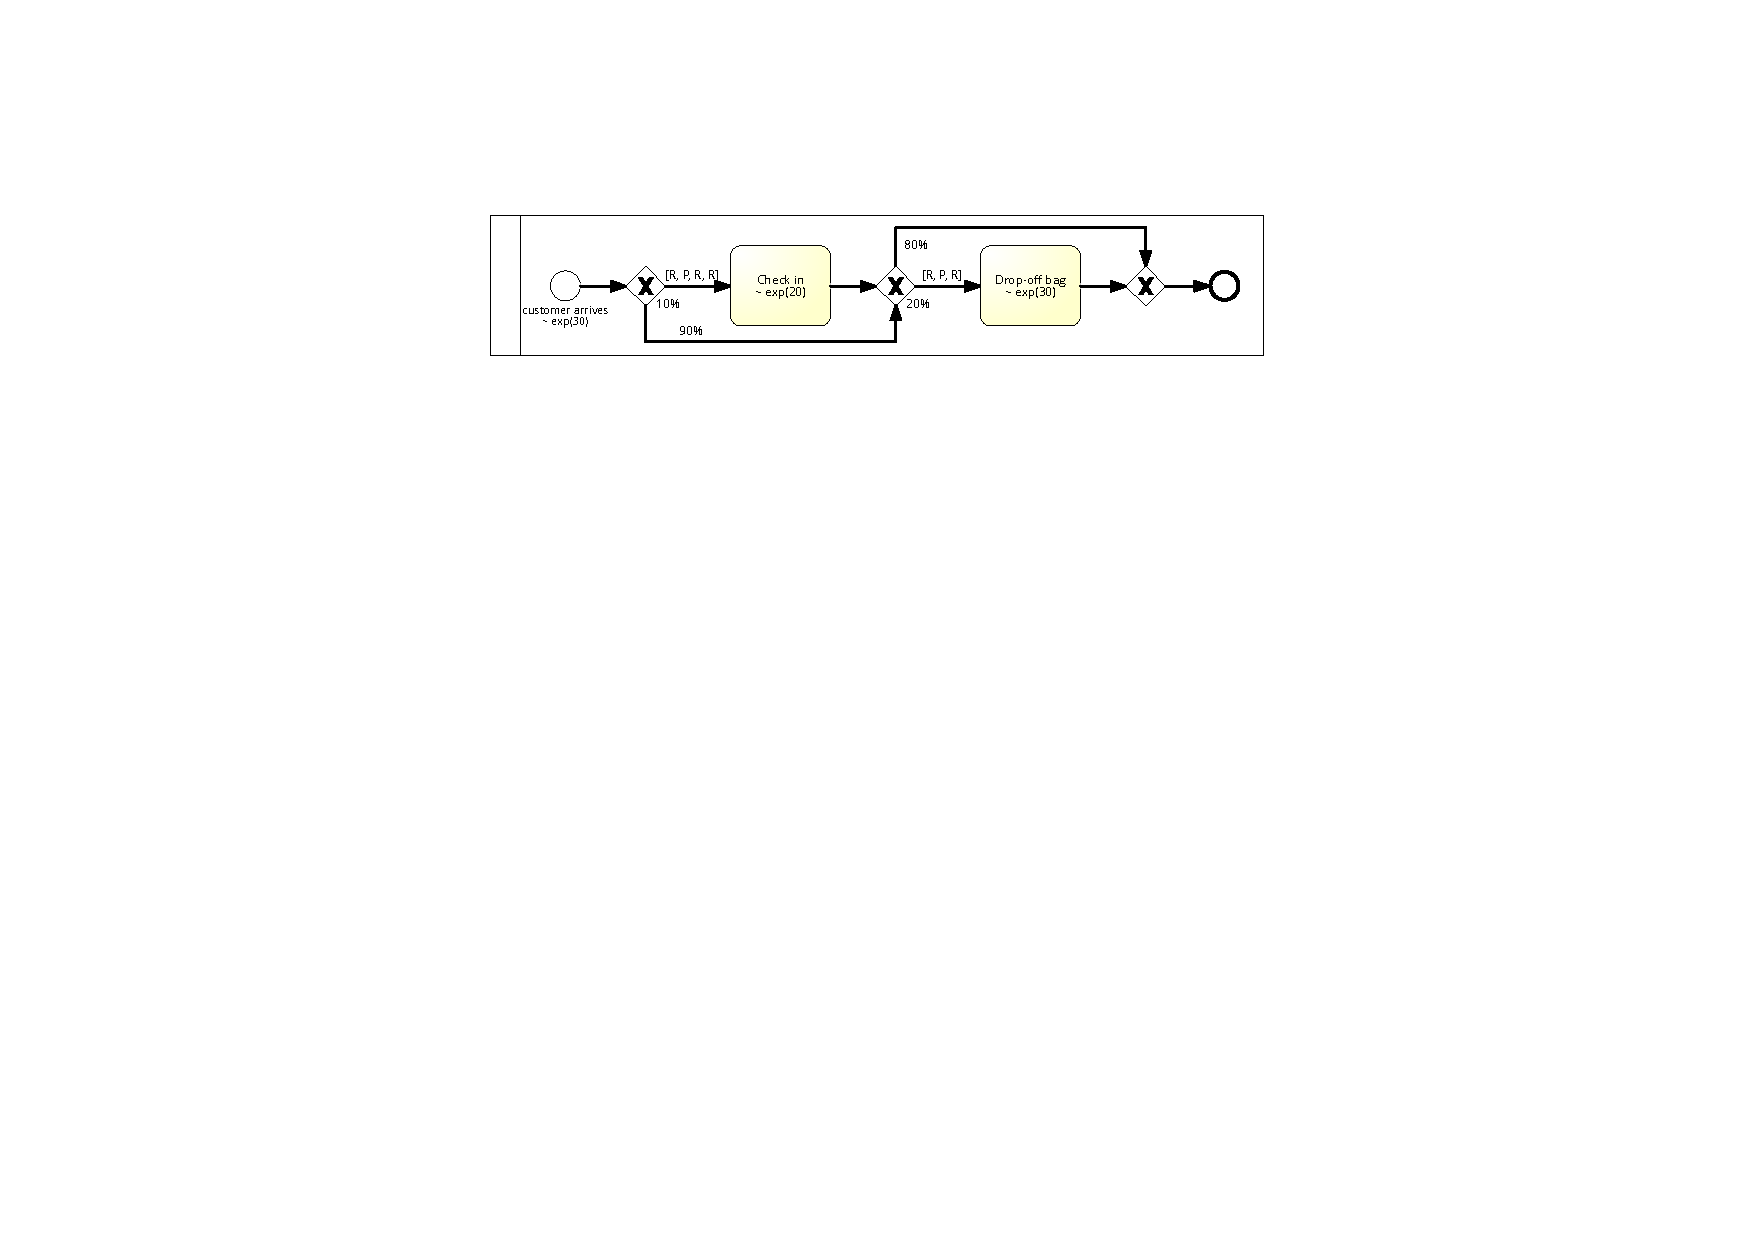
\includegraphics[width=1.0\linewidth]{figs/prio.pdf}
    \caption{Example of task prioritization.}
    \label{fig:prio}
\end{figure}
Task prioritization concerns the decision on the order in which tasks - or rather task instances - should be processed. This is particularly relevant when multiple task instances are waiting to be processed by the same resource. In that case, a decision must be made on which task instance should be processed first. This decision can be based on various criteria, such as minimizing the waiting time of customers or minimizing the waiting time of a specific type of resources. It may be subject to constraints, such as deadlines on specific task instances.
In other words, task prioritization selects the next work item to execute from a set of waiting work items (e.g., the next item in a shared worklist), potentially based on case attributes, due dates, or priority classes.

Figure~\ref{fig:prio} shows an example of a task prioritization. The process shows a check-in process at an airport, where customers arrive at a rate of 30 per hour (exponentially distributed). Arriving customers may need to check in, drop off a bag, both, or neither. The process illustrates that 10\% of the customers need to check in at the airport (the others have already done so at home) and 20\% needs to drop off a bag (the others only have carry-on luggage). The airline distinguishes between regular and priority customers. The task prioritization problem concerns the decision of the order in which the customers should be helped and the specific task that should be processed first. Figure~\ref{fig:prio} shows that in the current state of the process, there are four customers waiting for check-in (three (R)egular and one (P)riority) and three customers waiting to drop off a bag (two (R)egular and one (P)riority). The task prioritization problem concerns the decision on which of these seven task task instances should be processed first. This decision can be based on various criteria, such as minimizing the total waiting time of all customers or minimizing the waiting time of priority customers first and then the waiting time of regular customers.

Resource allocation concerns the decision on which resources should be assigned to which tasks. This is particularly relevant when multiple resources are available to perform a task, or when a resource can perform multiple tasks. The decision can be based on criteria such as minimizing the sum of processing times of tasks or minimizing the costs of using specific resources. It may be subject to constraints, such as resource availability, deadlines of cases, and budget limitations.
In other words, resource allocation selects a resource for a given work item (or, more generally, decides an assignment between a set of resources and a set of waiting work items), potentially based on skills, costs, and expected processing times.

Figure~\ref{fig:allocation} shows an example of a resource allocation problem. The process shows a loading process at a simple container terminal. Trucks arrive at the container terminal at a rate of 10 per hour (exponentially distributed). There are two types of trucks (T1 and T2) and two cranes. The loading times depend on both the type of truck and the crane that is used. Figure~\ref{fig:allocation} shows that in the current state of the process, there are five trucks waiting: three of type T1 and two of type T2. Both cranes are available. We assume that trucks are handled in the order of their arrival (i.e., task prioritization is done on a first-come-first-served basis). Consequently, the next truck to be handled is a truck of type T2. What remains is the decision on which crane should be assigned to this truck. This decision can be based on various criteria, such as minimizing the total processing time of all trucks.

\begin{figure}[t!]
    \centering
    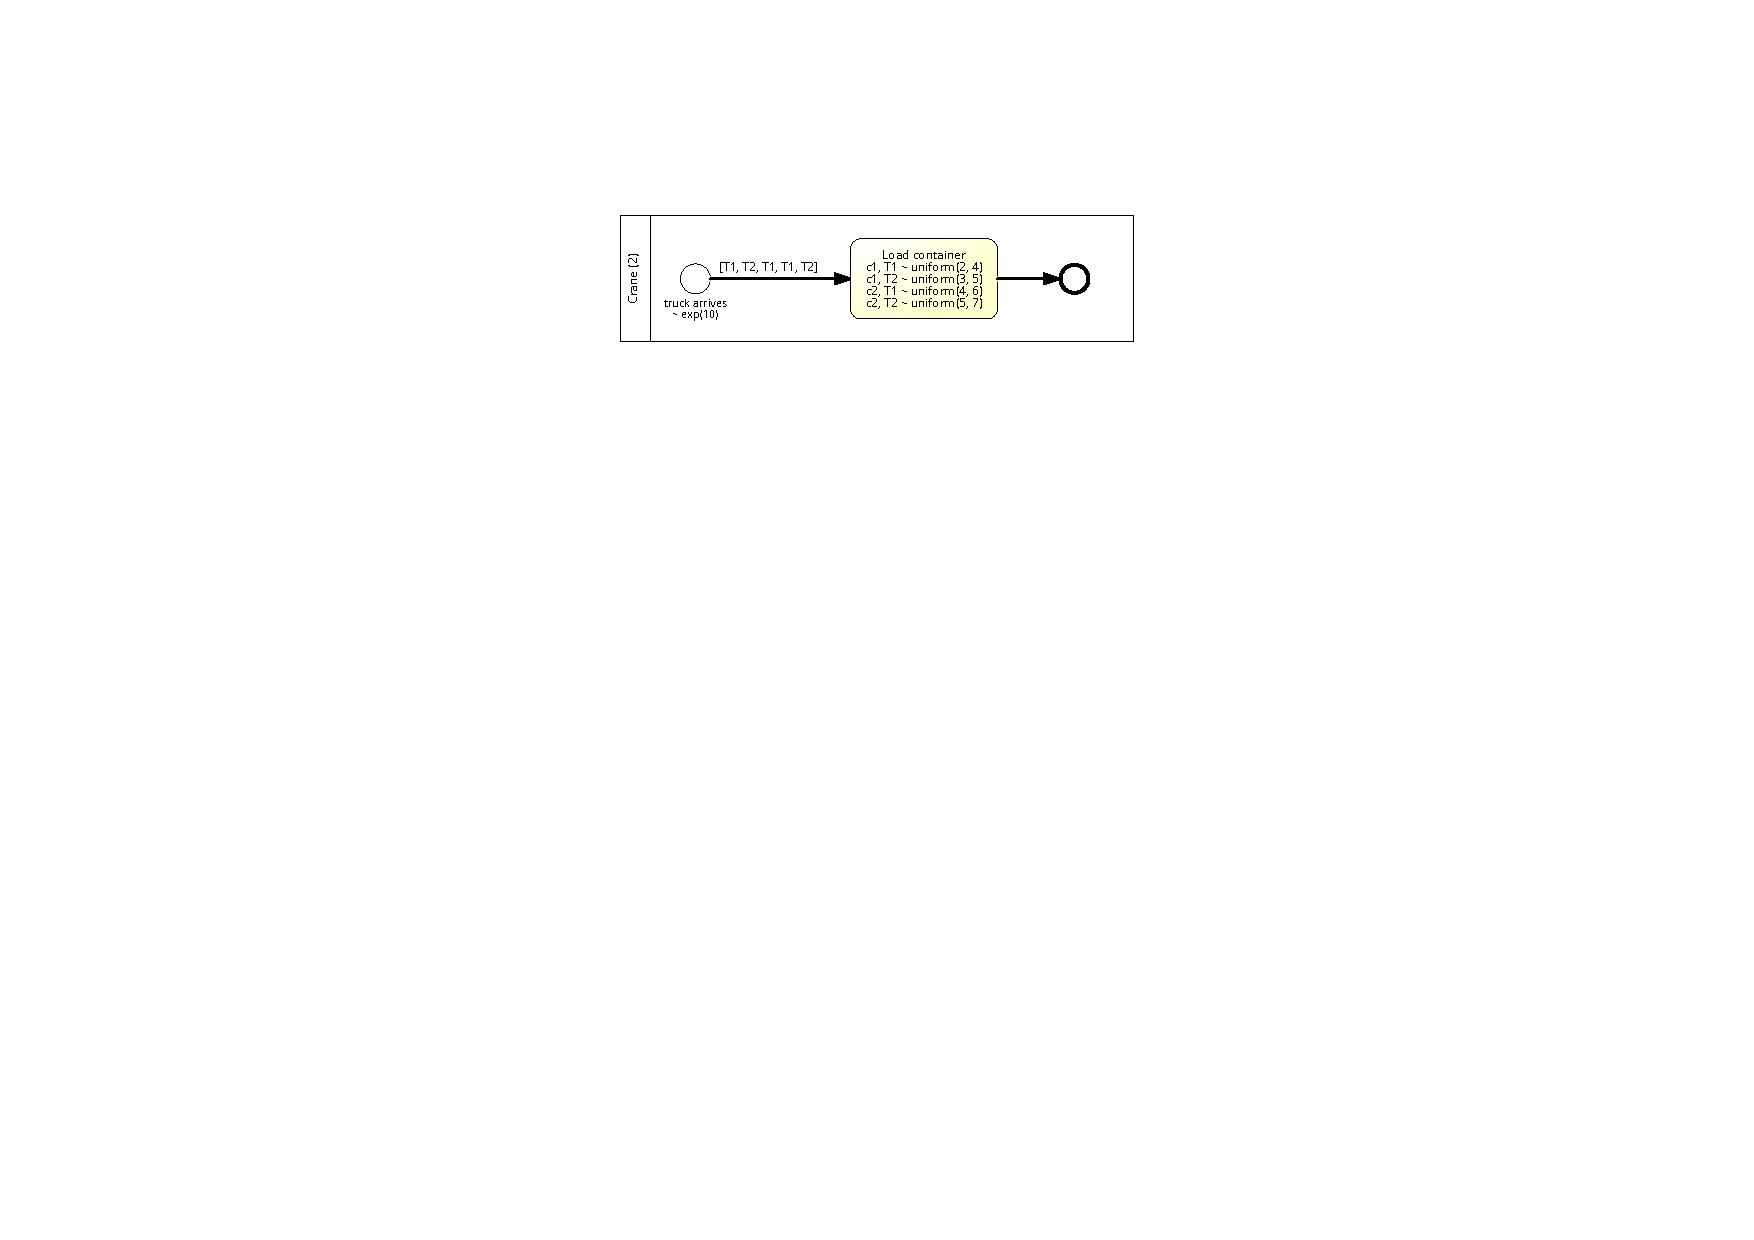
\includegraphics[width=0.9\linewidth]{figs/allocation.pdf}
    \caption{Example of resource allocation.}
    \label{fig:allocation}
\end{figure}

It is common for the task prioritization and the resource allocation problems to be combined. In that case, the decision that must be made concerns both the order in which tasks should be processed and the resources that should be assigned to these tasks. In Figure~\ref{fig:allocation}, this would mean that the decision concerns both which of the five waiting trucks should be processed next and which crane should be assigned to this truck.
In the operations literature this combined decision is often referred to as (dynamic) dispatching or task allocation.


\subsection{Case Admission and Scheduling}

Case admission and scheduling concerns the decision on whether and when a case should be released into a process (or into a specific stage of a process). This includes decisions that set an explicit appointment time, but may also include decisions that delay or reject cases when capacity is limited. The decision can be based on criteria such as minimizing waiting time, meeting due dates, or maximizing the utilization of resources, subject to constraints such as resource availability, deadlines, and budget limitations.

Figure~\ref{fig:admission} shows an example of an admission control problem. The process shows a garage that services cars. The garage receives calls from customers at a rate of 5 per hour. When a customer calls, a planner decides when to plan the maintenance on the car of the customer. The process then pauses and continues at the planned time, upon which the maintenance is performed by one of the five mechanics that work at the garage.

\begin{figure}[t!]
    \centering
    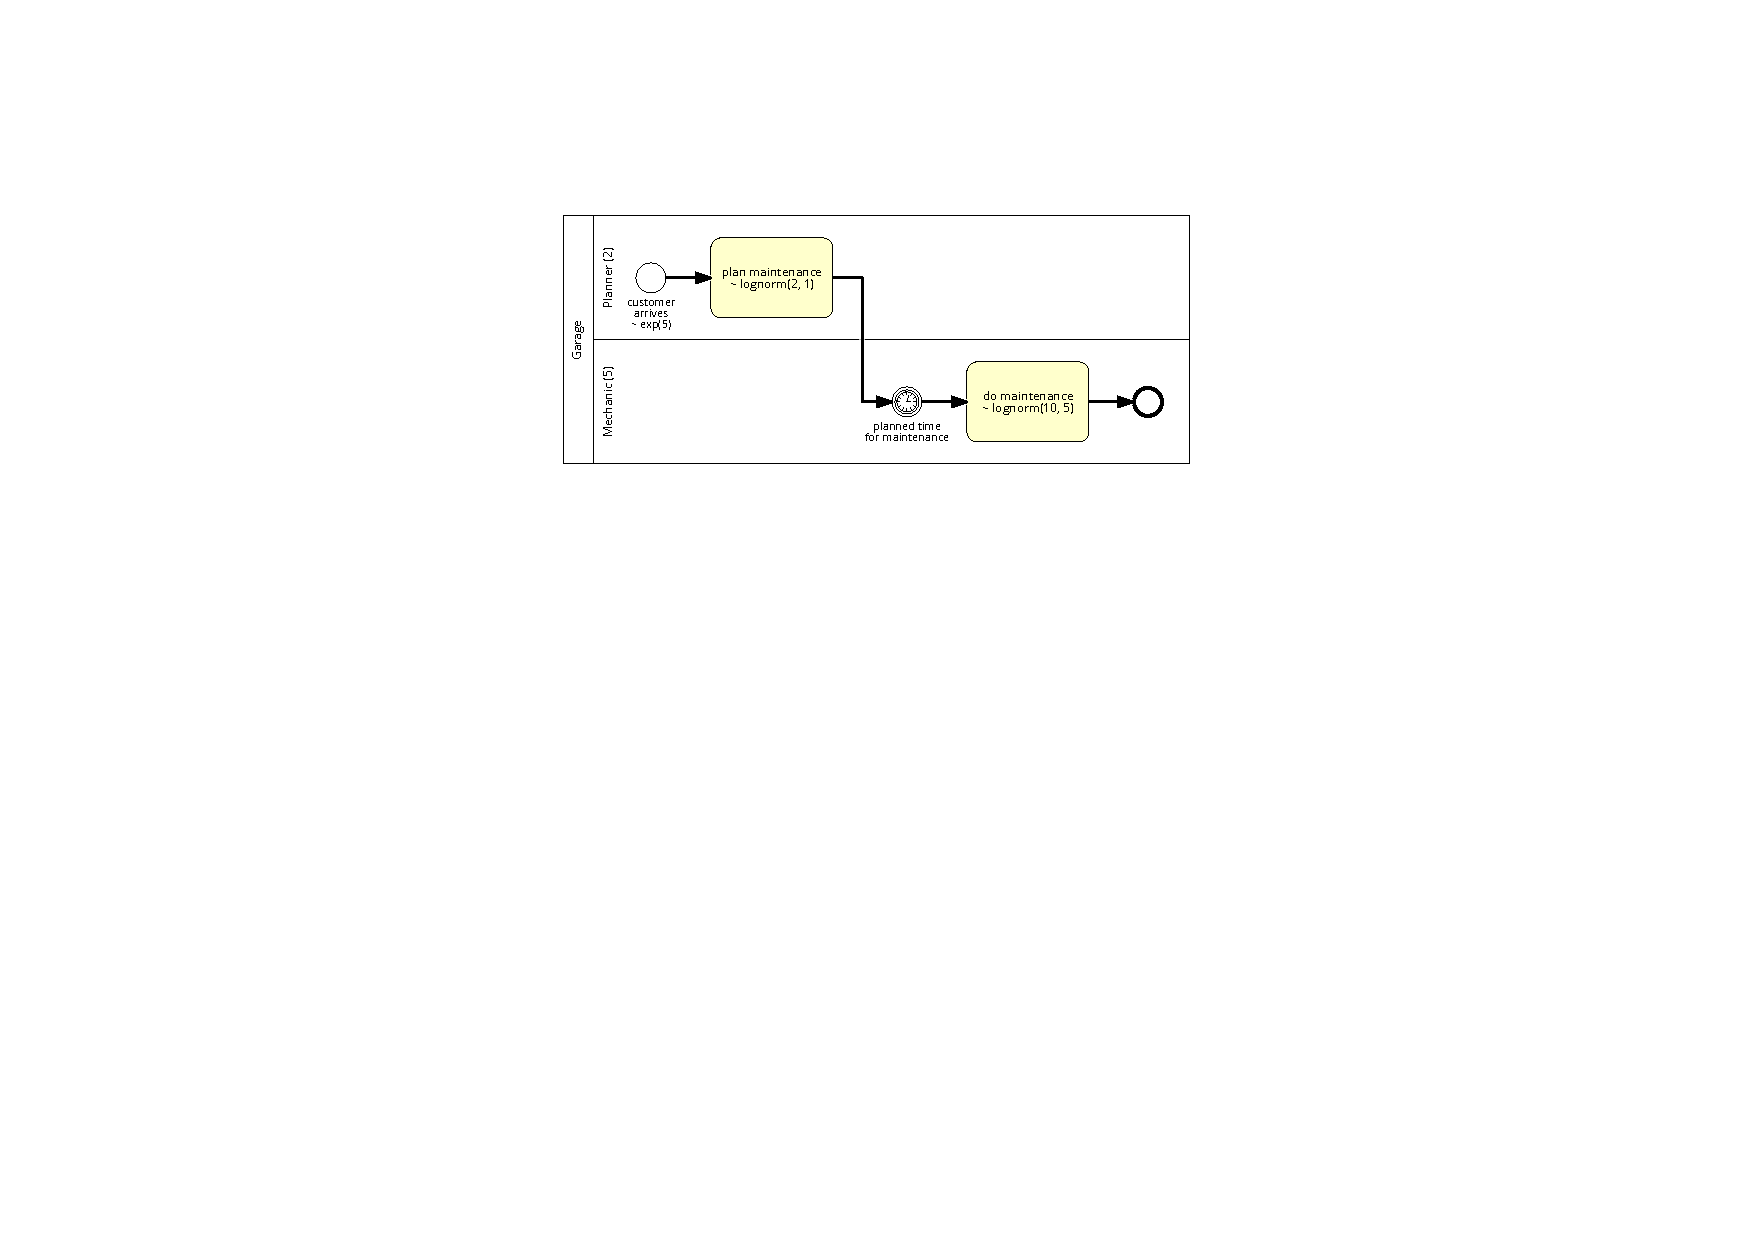
\includegraphics[width=1.0\linewidth]{figs/admission.pdf}
    \caption{Example of admission control.}
    \label{fig:admission}
\end{figure}


\subsection{Staffing}

Staffing concerns the decision on how many resources of which type should be scheduled to work at which time. This decision can be based on criteria such as minimizing the cost of resources or maximizing the number of customers that can be served. It may be subject to constraints, such as resource availability and budget limitations.
In contrast to resource allocation, staffing changes the available capacity over time (e.g., through shifts, call-ins, cross-training, or temporary capacity changes), rather than assigning an existing resource to a specific work item.

Figure~\ref{fig:staffing} shows an example of a staffing problem. The figure shows a process at a simple warehousing facility. At the warehouse, trucks arrive at a rate of 15 per hour (exponentially distributed). 50\% of the trucks are inbound truck that need to be unloaded and 50\% are outbound trucks that need to be loaded. There are eight resources in the warehouse, which can either take the role of inbound or outbound operator. Switching between these roles is possible, but takes time, because the employee needs to check the transportation order and decide on the best way to load or unload the truck, such that it is balanced and can be processed efficiently. Consequently, depending on the number of inbound and outbound trucks that are currently waiting and are expected to arrive, a decision must be made on how many resources should be assigned to work as inbound operators and how many as outbound operators. This can be based on criteria such as minimizing the total waiting time of trucks.

\begin{figure}[htb]
    \centering
    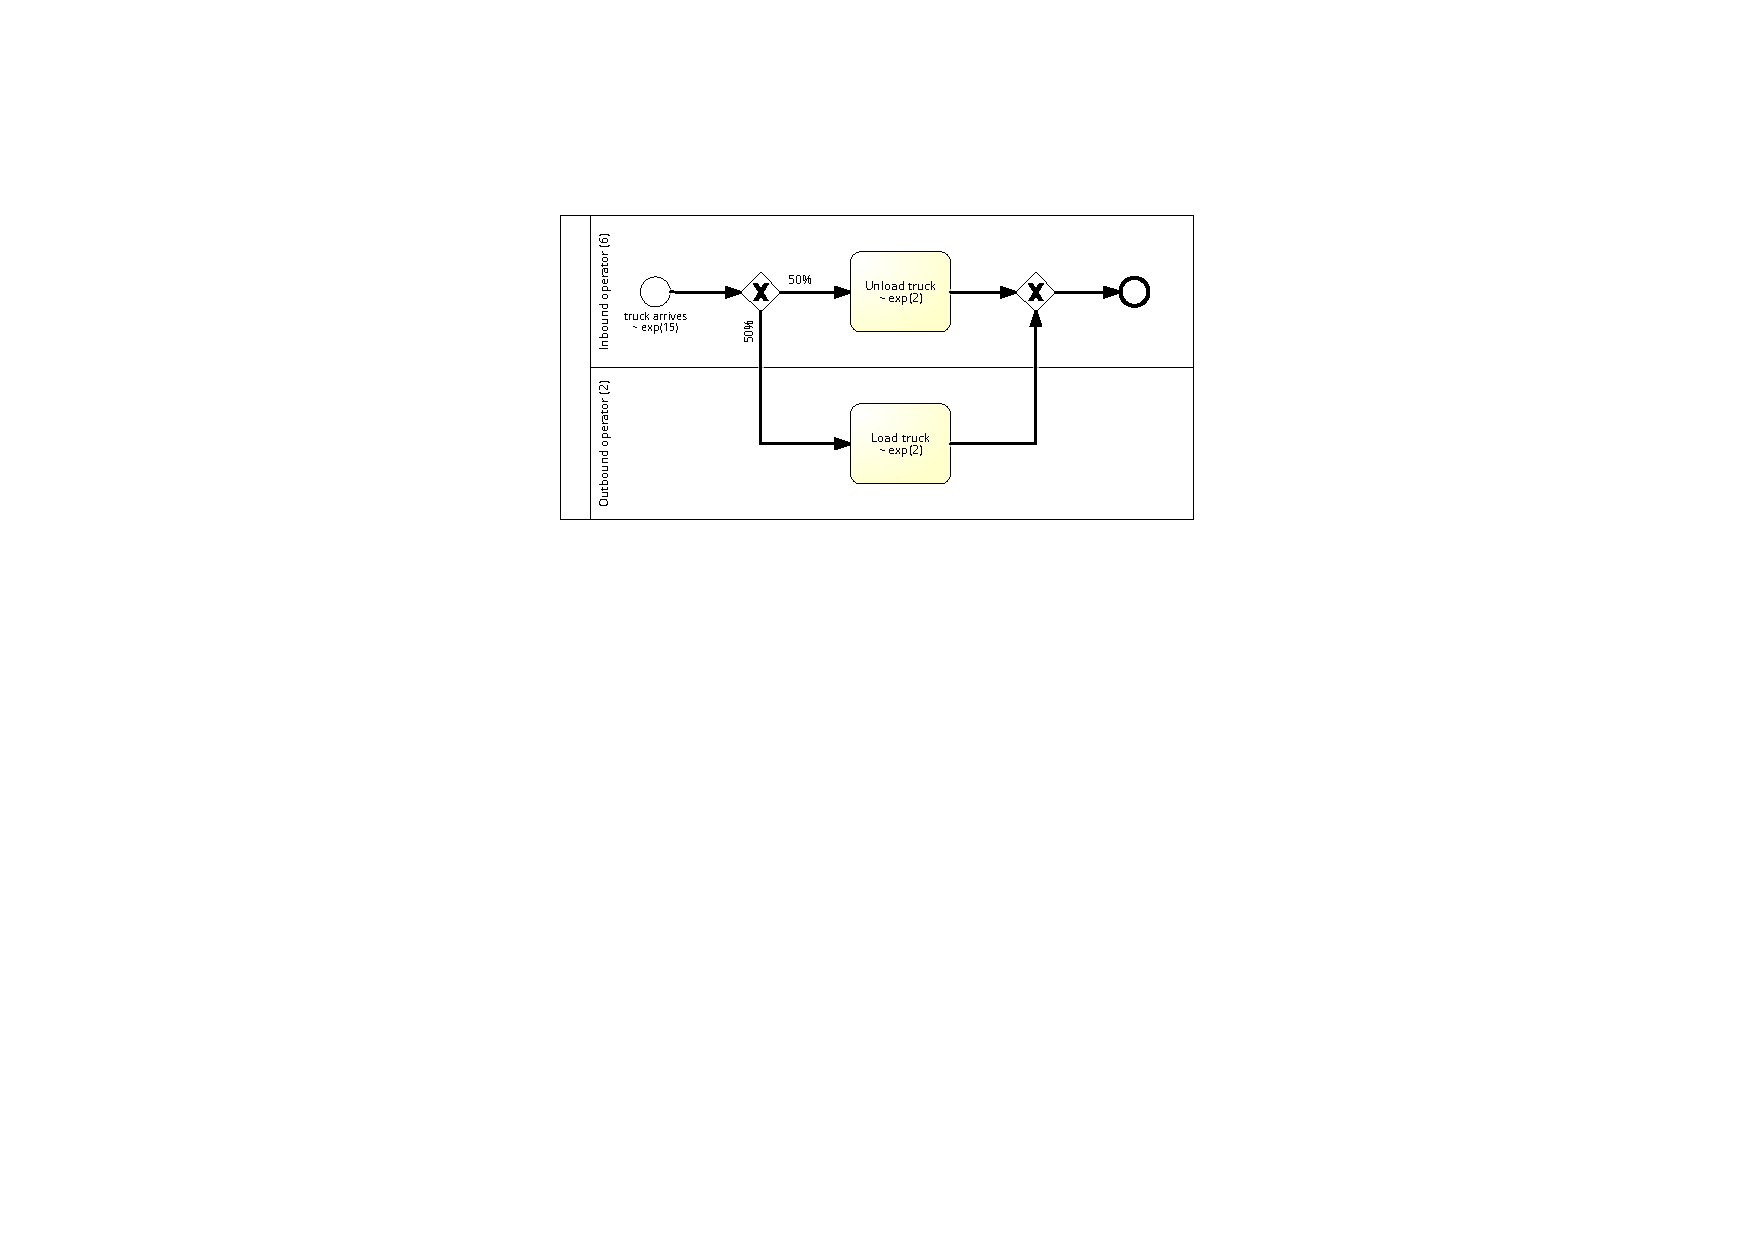
\includegraphics[width=1.0\linewidth]{figs/staffing.pdf}
    \caption{Example of staffing.}
    \label{fig:staffing}
\end{figure}


\subsection{Path Choice}

Path choice concerns the decision on which path a specific case should take through the process. This is particularly relevant when multiple paths are available to process a case, for example when a doctor can choose between different care pathways or when a customer service official can choose between different ways of processing a service request. The decision can be based on criteria such as minimizing the processing time of cases or optimizing the desired outcome of the process for a customer. It may be subject to constraints, such as which option is open to which type of case.
Path choice decisions are often state-dependent, and they may affect downstream outcomes (e.g., quality, rework probability, or failure probability), which creates a trade-off between immediate effort and expected future work.

Figure~\ref{fig:path_choice} shows an example of a path choice problem. The process shows a simple production process. In the process, production orders arrive at a rate of 1 per hour. When production starts, the core component must be staged. If the staging is not done well, the production operator may choose to redo the staging. After the staging is completed, the product is assembled and subsequently tested. If the test fails, the product must be reworked. The path choice problem concerns the decision on whether to redo the staging or not. This decision can be based on various criteria, such as minimizing the total processing time. The decision to redo the staging has impact on the processing time of the production order, because redoing the staging takes time, but it may also reduce the likelihood that the test will fail, which ends up taking even more time.

\begin{figure}[t!]
    \centering
    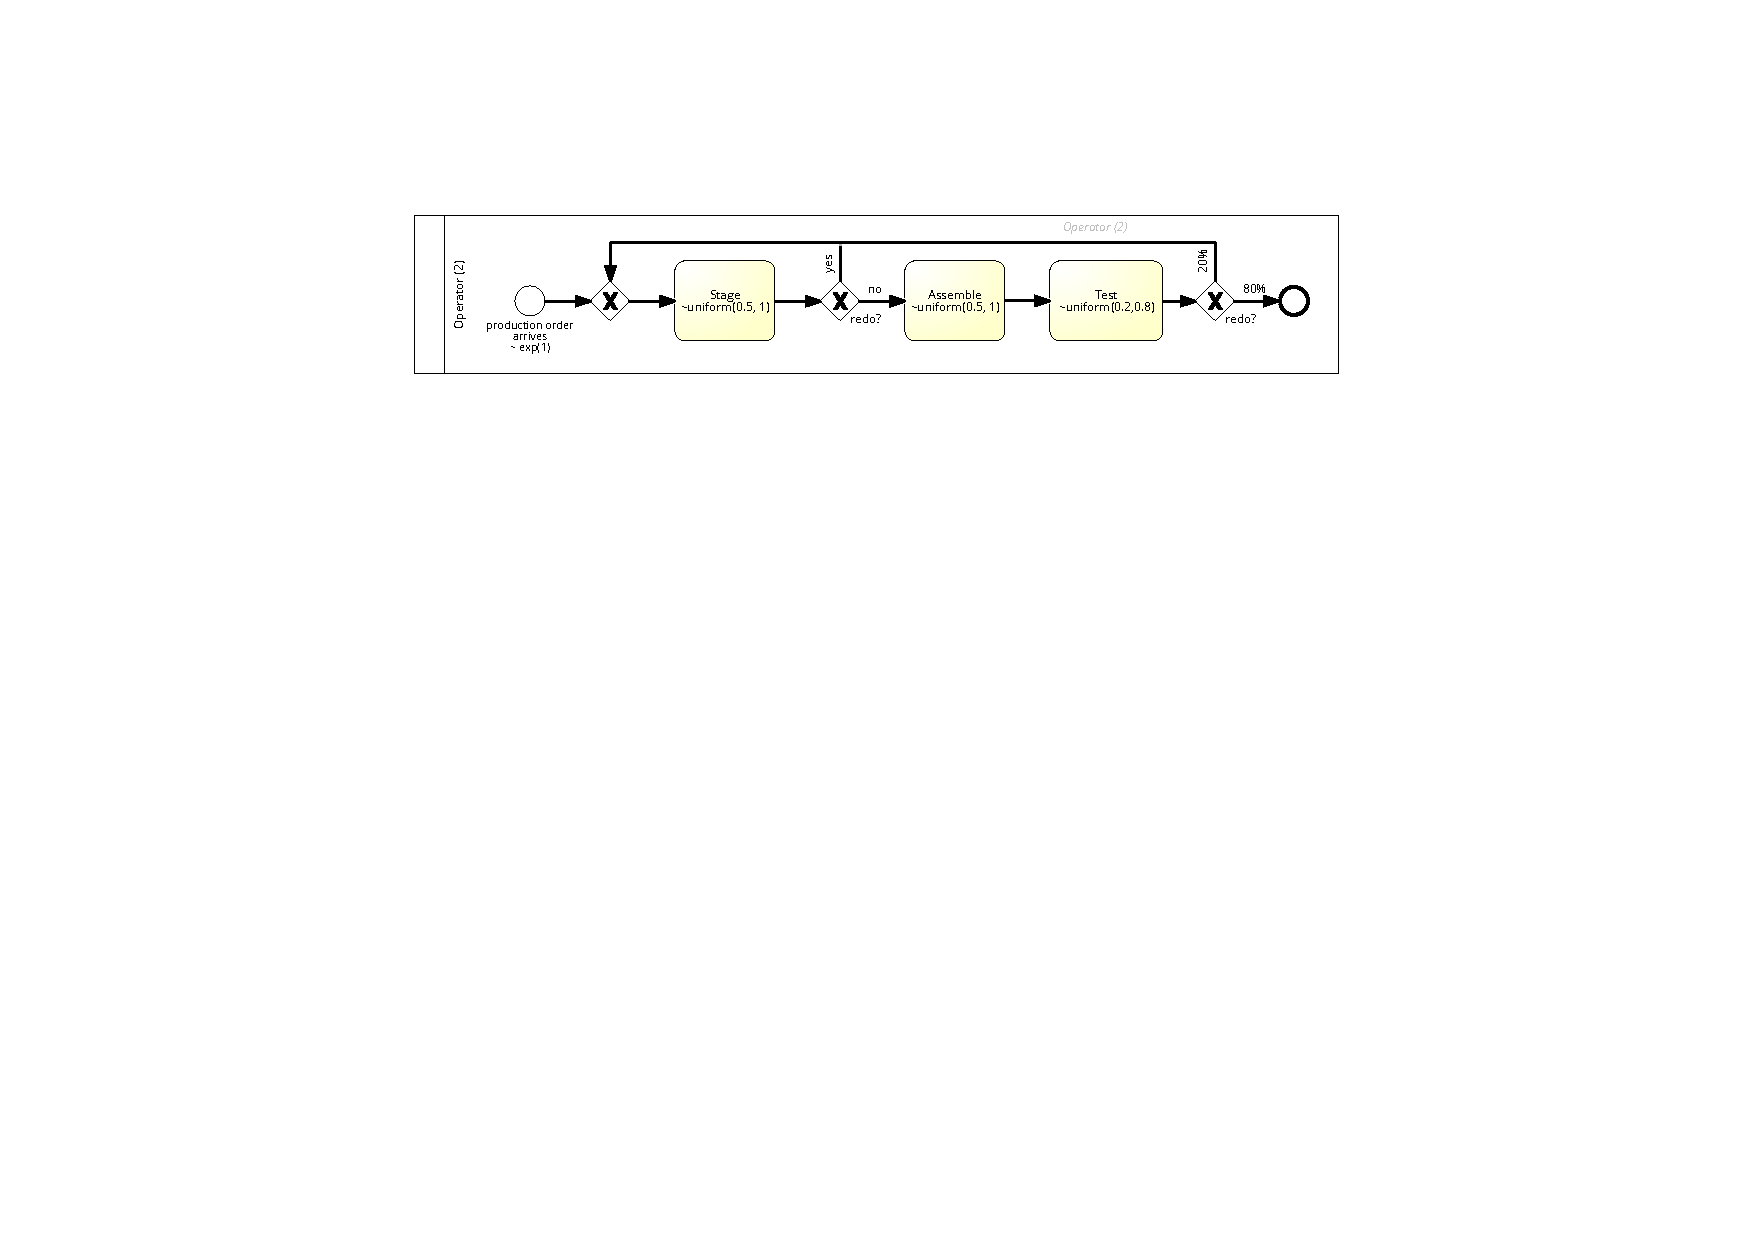
\includegraphics[width=1.0\linewidth]{figs/choice.pdf}
    \caption{Example of path choice.}
    \label{fig:path_choice}
\end{figure}

The above taxonomy is not intended to be exhaustive. Additional families of BPO decision-making problems include batching decisions (when to group cases), promise and escalation decisions (how to set and manage service levels and due dates), process variant selection (which process configuration to use for a case or for a period), and information acquisition decisions (which checks or measurements to perform to reduce uncertainty before committing to an action).


\subsection{Operational, Tactical, and Strategic Variants}

The previous sections presented different types of BPO decision-making problems at an operational level, meaning that the decisions concern individual cases and resources during the execution of the process and are made in real-time as new cases arrive. Each of these problem types has counterparts at a tactical and strategic level as well. These levels differ in time horizon and scope. Strategic decisions are long-term and focus on the overall direction and structure of the process (e.g., policies, roles, and process design). Tactical decisions are medium-term and focus on planning and scheduling (e.g., shift scheduling or batch planning). Table~\ref{tab:levels} shows an overview of different types of BPO decision-making problems at the operational, tactical, and strategic levels.
\begin{table}[t]
\caption{Optimization problems at different levels}
\label{tab:levels}
\small
\setlength{\tabcolsep}{6pt}
\renewcommand{\arraystretch}{1.25}
\begin{tabularx}{\textwidth}{
  @{}
  l
  >{\raggedright\arraybackslash}X
  >{\raggedright\arraybackslash}X
  >{\raggedright\arraybackslash}X
  >{\raggedright\arraybackslash}X
  @{}
}
\toprule
\textbf{Level} &
\textbf{Task Prioritization \& Resource Allocation} &
\textbf{Case Admission \& Scheduling} &
\textbf{Staffing} &
\textbf{Path Choice} \\
\midrule
\textbf{Strategic} &
Role / worklist design &
Admission and schedule rule design &
Workforce size and skill mix design &
Process (re)design \\

\textbf{Tactical} &
Task scheduling &
Scheduling &
Shift scheduling &
Policy setting \\

\textbf{Operational} &
Task allocation &
Admission control &
Dynamic capacity control &
Case routing \\
\bottomrule
\end{tabularx}
\end{table}


The strategic level concerns decisions regarding the design of the process itself. This includes the design of the control-flow of the process, but as business process optimization is concerned, it also concerns the design with respect to other aspects of the process, especially the types and numbers of employees and other resources that are involved in the process and the rules that govern their deployment. 

At this level, the task prioritization and resource allocation problems are typically combined. Decisions regarding task prioritization and resource allocation at a strategic level concern the design of roles and worklists. Roles determine which types of employees are distinguished in the process and which tasks they are allowed to perform. Worklists determine the rules that govern the order in which tasks are performed and by whom they are performed. For example, a worklist may be defined such that all employees (in an authorized role) can freely choose which task they want to perform from that worklist. Alternatively, worklists can be defined per employees, in which tasks appear in order of their priority or where even only the next task to be performed appears. These two mechanisms represent widely different ways of organizing the work and can have a very different impact on the performance of the process, but also the job satisfaction of the employees as they are more of less free to organize their work as they see fit. Many alternative worklist designs can be envisioned as well. Decisions regarding case admission at a strategic level concern the design of admission rules, such as first-come-first-served or priority-based admission. Decisions regarding staffing at a strategic level concern the design of the staffing structure, such as the types and numbers of employees that are involved in the process.

The tactical level concerns decisions regarding the planning and scheduling of cases, resources, and tasks ahead of time and for a longer timeframe than the operational level. At this level, the task prioritization and resource allocation problems are typically combined as well. Decisions regarding task prioritization and resource allocation at a tactical level are typically taken for a longer period of time, such as a day or a week. This implies that their scheduling is often done in batches and at fixed points in time. For example, task scheduling may be done once per day at the end of the day for all tasks that are still open. At that time, a scheduling algorithm can determine for each open task when it should be processed and by whom. Note that there is a relation between task scheduling and task allocation: ideally, at an operational level task allocation decisions simply follow the schedule that is made at a tactical level. However, this is not always possible, because the situation at the operational level may differ from what was expected at the tactical level. For example, a resource that was scheduled to work may be sick or a task may take much longer than expected. In that case, the task allocation decision at the operational level must deviate from the schedule that was made at the tactical level. Still, the schedule made at the tactical level can serve as a guideline for taking decisions at the operational level. Admission scheduling is similar to task scheduling, but concerns the scheduling of the admission of a case rather than scheduling of individual tasks in that case. However, like task scheduling, it is typically done in batches, at fixed points in time, and concerns the decision on when to admit which case for further processing. Also, like task scheduling, there is a strong relation between case scheduling and case admission control at the operational level, in that case scheduling decides on an ideal admission time for each case, which serves as a guide for admission control. While admission control may deviate from the schedule if necessary, for example when a case is late or cancelled. Staffing at a tactical level concerns the scheduling of shifts for employees. This typically involves determining how many employees of which type should be scheduled to work during specific shifts. This decision is again similar to task and case scheduling in that it is typically done in batches, at fixed points in time, and is related to ad-hoc resource scaling at the operational level.


\section{A Framework for Business Process Optimization}\label{sec:framework}

To solve a BPO decision-making problem, a solution approach must be designed. Figure~\ref{fig:framework} presents the core components that are typically involved in solving a BPO problem.

\begin{figure}[t!]
    \centering
    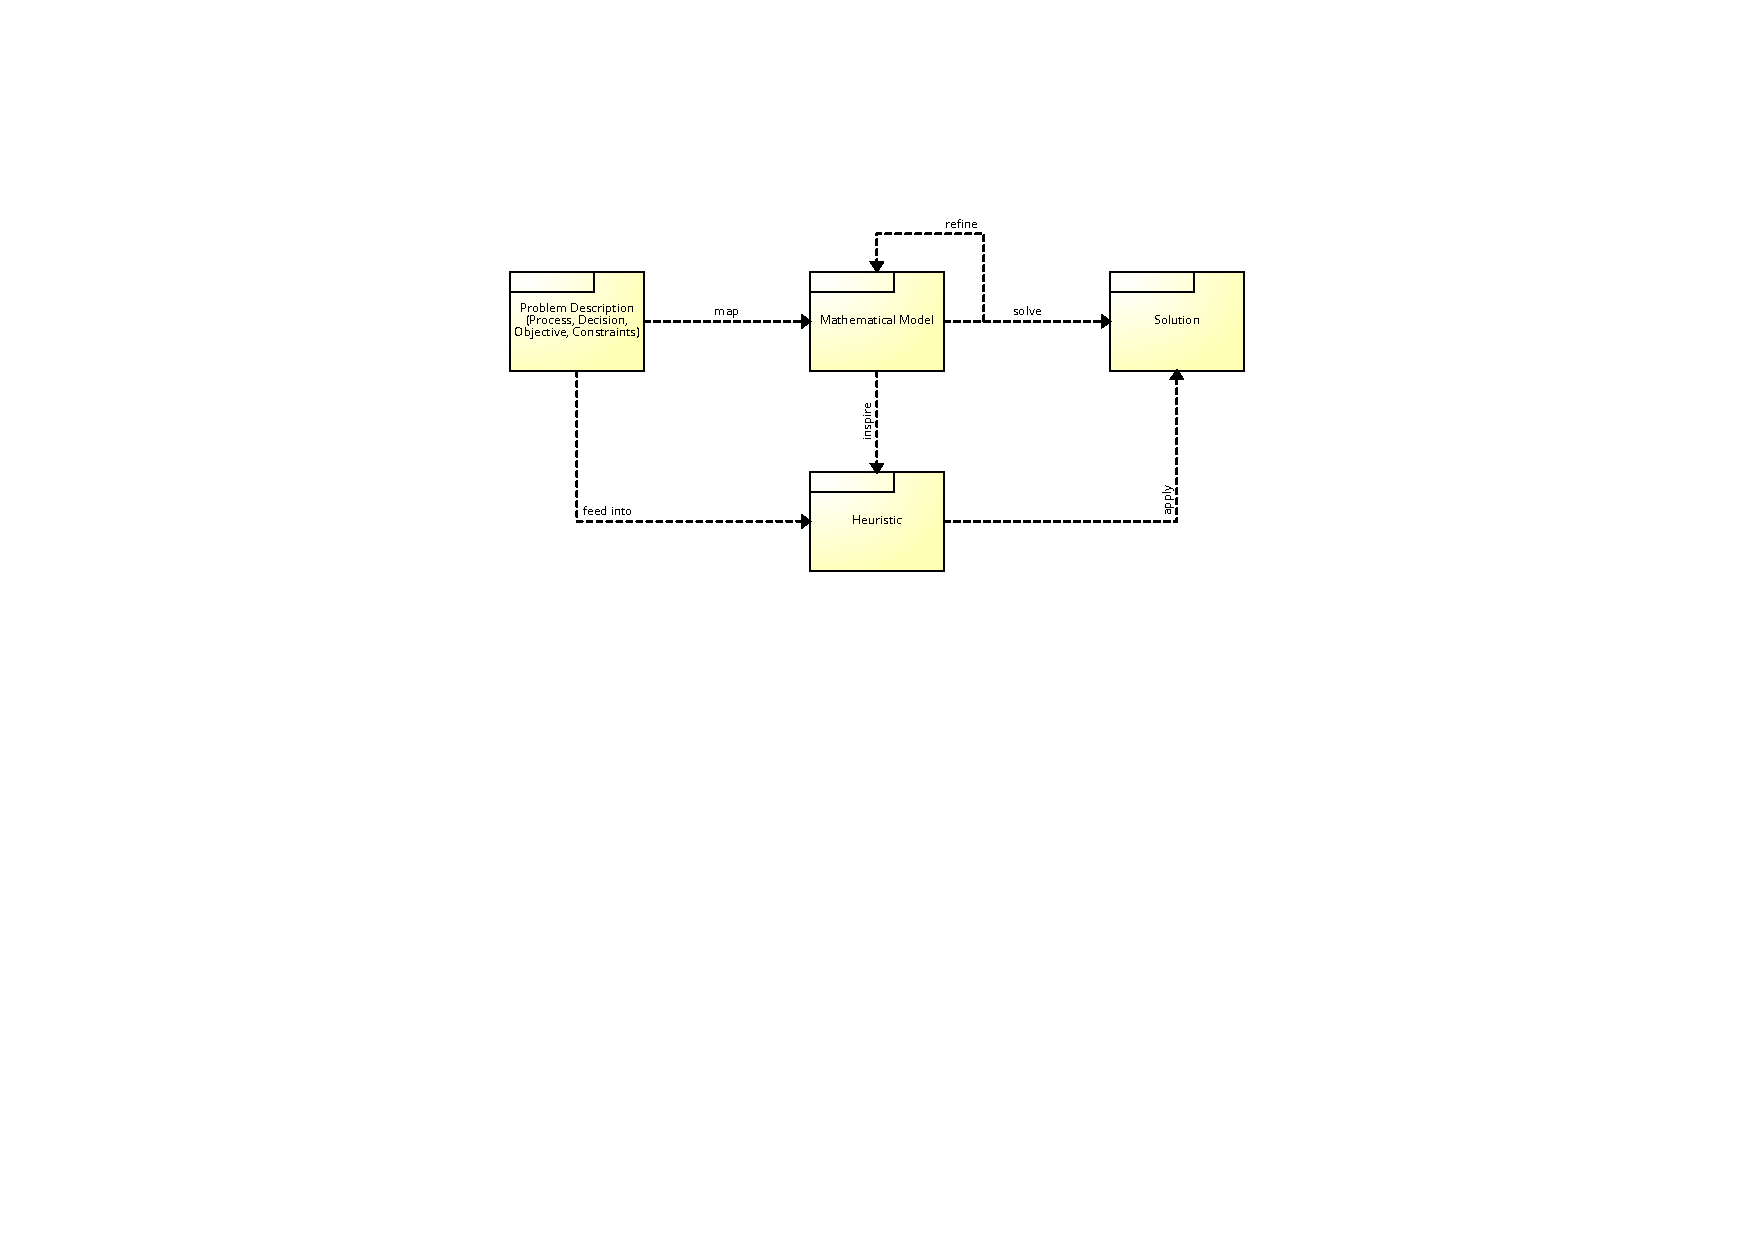
\includegraphics[width=1.0\linewidth]{figs/framework.pdf}
    \caption{A framework for business process optimization.}
    \label{fig:framework}
\end{figure}

The first component is the \textbf{problem definition}, which defines the BPO decision-making problem that needs to be solved. For a business process optimization problem, this involves the definition of the process that must be optimized. However, as with any optimization problem, this must also include the decision that must be made, the objective(s) that need to be optimized, and the constraints that must be satisfied. For tactical and operational BPO problems, the problem definition also typically includes the current state of the process, such as the cases that are currently being processed and the resources that are currently available. For example, for the resource allocation problem in Figure~\ref{fig:allocation}, the problem definition includes the process model, the decision on which crane should be assigned to the next truck, the objective to minimize the total processing time of all trucks, and the constraint that only one crane can be assigned to at most one truck at a time. It also includes the current state of the process, which shows that there are five trucks waiting and both cranes are available.

In addition, BPO problems are typically defined under uncertainty, for example in case arrivals, activity durations, and the paths that cases take. In practice, this often requires a \textbf{data and uncertainty model} that specifies how uncertain quantities are represented and, when applicable, how they are estimated from historical event logs (e.g., through prediction models for remaining time, rework probability, or outcomes).

The second component is an optional \textbf{mathematical model}, which defines the problem in mathematical terms. This is not always necessary, but it can be useful to gain a better understanding of the problem or to apply mathematical optimization techniques. The mathematical model must be constructed based on the problem definition. Several modeling paradigms are used in BPO, including mathematical programming formulations (e.g., Mixed Integer Programming (MIP), constraint programming, and stochastic programming), analytical models (e.g., queueing-based models), and sequential decision models (e.g., Markov Decision Processes (MDPs)). For example, for the resource allocation problem in Figure~\ref{fig:allocation}, a MIP can be constructed, including binary decision variables that indicate whether a specific crane is assigned to a specific truck, an objective function that minimizes the total processing time of all trucks, and constraints that ensure that each truck is assigned to at most one crane and each crane is assigned to at most one truck at a time. This mathematical model can then be solved using a MIP solver, such as CPLEX or Gurobi. Sometimes, the mathematical model can be solved directly to obtain an optimal solution. However, for many BPO problems, the mathematical model is too complex to be solved directly. In that case, the mathematical model can be refined to make it easier to solve. Alternatively, it can serve as a basis for designing a heuristic.

The way in which solutions are applied also differs across BPO settings. \textbf{Offline (periodic) optimization} computes decisions for a planning horizon (e.g., staff rosters, appointment schedules, or batch plans) and is typically re-run at fixed times. \textbf{Online (real-time) optimization} takes decisions during execution, conditioned on the current process state (e.g., dispatching, routing, and admission control). Both settings share the same core components in Figure~\ref{fig:framework}, but they differ in the frequency of decision-making, the amount of uncertainty that is resolved between decisions, and the way solutions are evaluated.

A \textbf{heuristic} defines a set of rules or guidelines to solve the problem. The heuristic must be designed based on the problem definition and can be inspired by a mathematical model of the problem (if available). A heuristic takes the current state of the process as input and produces a solution as output. Heuristics can be simple or complex, depending on the problem and the desired quality of the solution. For example, for the resource allocation problem in Figure~\ref{fig:allocation}, a simple rule-based heuristic is to use, in each state, the allocation of a crane to a truck that has the shortest expected processing time. For this specific problem, this heuristic provides an optimal solution; that is, it achieves the objective of the problem in that it minimizes the total processing time of all trucks. However, for many BPO problems, such simple heuristics do not provide an optimal solution. In that case, more complex heuristics can be designed, or more complex solution methods---based on mathematical models---can be used.

Whether by solving a mathematical model or by applying a heuristic, the method produces a \textbf{solution} to the problem. The solution consists of the decision that must be made. For example, for the resource allocation problem in Figure~\ref{fig:allocation}, the solution consists of the decision on which crane should be assigned to the next truck. Note that an evaluation component is typically required to assess a solution approach. Depending on the setting, evaluation may rely on analytical performance measures, simulation (e.g., what-if analysis and digital twins), or event-log replay. 

In the remainder of this paper, we use this framework to (i) define a vocabulary for describing BPO problems precisely (Section~\ref{sec:problemdescription}), (ii) structure typical families of solution approaches (Section~\ref{sec:solutionapproaches}), and (iii) organize representative problem--solution pairs from the literature (Section~\ref{sec:survey}).

\section{Problem Description}\label{sec:problemdescription}

To provide a problem description, we need a vocabulary. We will use the concepts from the meta-model in figure~\ref{fig:metamodel} for those purposes. The part above the dotted line defines concepts for describing the process, and the part below the dotted line defines the concepts for describing the state of the process. The concepts for describing the process are summarized from the BPMN standard and can, therefore, be used to describe BPMN models. For example, in figure~\ref{fig:allocation}, there is an event named `truck arrives', a task named `load container', a flow from `truck arrives' to `load container', and a lane `Crane' that is authorized for `load container'. The state of a process is defined by two concepts. One describes the cases that are executed by the process, and the second describes the resources. Cases can be waiting (in a queue) for a node, such as a task or an intermediate event. A resource can also be executing a task for them. For example, in in figure~\ref{fig:allocation}, there are two resources, c1 and c2, and there are five cases waiting for the task `load container. There are no tasks being executed.

\begin{figure}[htb]
    \centering
    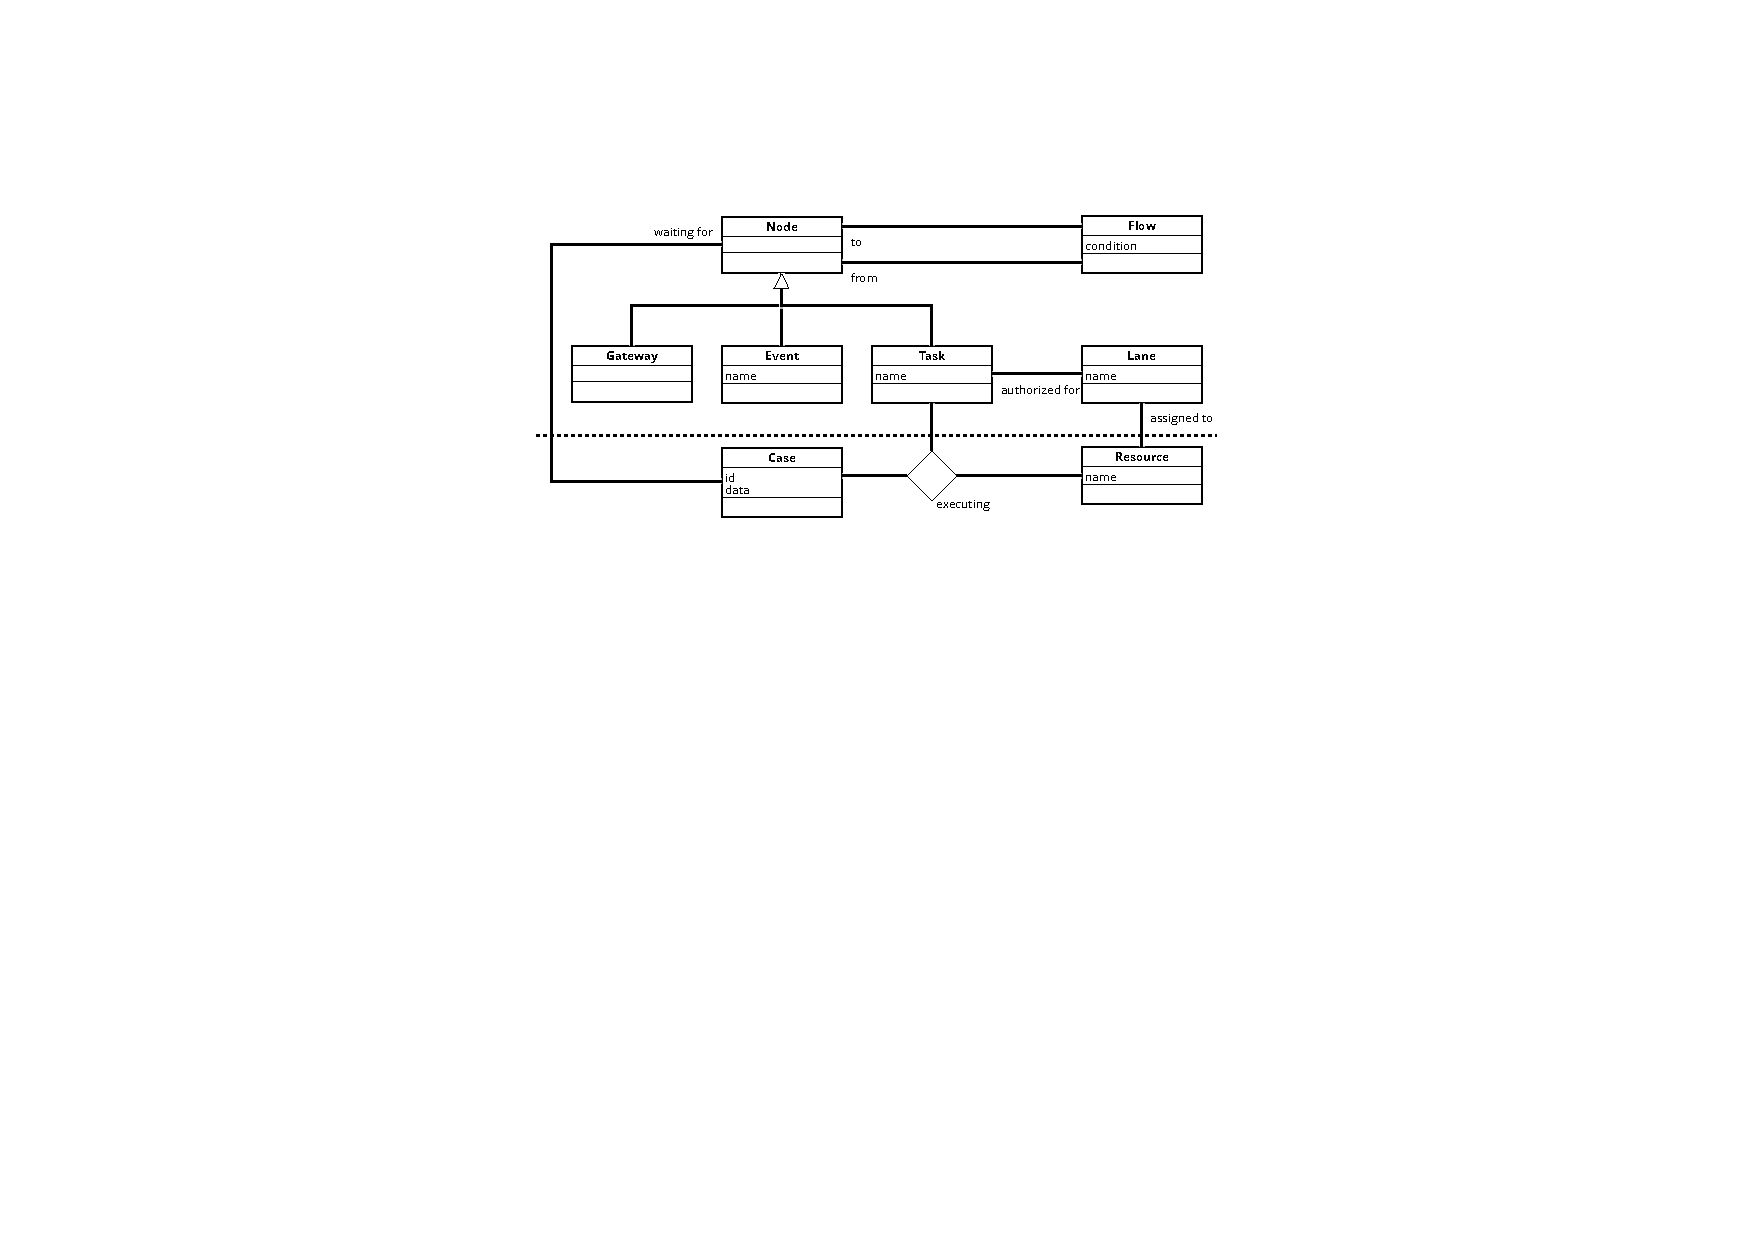
\includegraphics[width=1.0\linewidth]{figs/metamodel.pdf}
    \caption{A meta-model for problem descriptions.}
    \label{fig:metamodel}
\end{figure}

To be able to provide a mathematical definition of a problem, we will also interpret classes from the meta-model as sets, associations as sets of tuples, and attributes as functions that assign values to objects of classes. When there can be no confusion, we will also refer to objects by their attributes. For example, in figure~\ref{fig:allocation}, there are two resources. Let's call them `r1' and `r2' and there is a function `name' that maps $\{r1\mapsto c1, r2 \mapsto c2\}$. Since the name also uniquely identifies the resources, we will simply refer to the resources as `c1' and `c2'. As another notational convenience, we will also use the `.' to refer to the attribute or the associated objects of an object. For example, `c1.assigned to' is the lane `Crane', or - strictly speaking - the set of lanes with the single element $\{Crane\}$. We also allow the dot notation to be applied to sets, by simply applying it to each element of the set, and - as in the previous line - if there can be no confusion, we do not distinguish between the singleton set and its element. For example, we can also refer to `c1.assigned to.authorized for.name', which would return the singleton set $\{load\ container\}$. Since this is a singleton set, we will also simply refer to `load container'.

These concepts - and their set-theoretic counterparts - will allow us to define business process optimization problems precisely. Each BPO problem description has five elements:
\begin{compactitem}
    \item The process, which defines the tasks that can be executed for cases, the resources that can execute those tasks, as well as how the process progresses from one state to the next.
    \item The decision moments, which is a condition over the states of a process that expresses in which states the a decision needs to be taken. This condition can be as simple as `each day at 2:00 AM'. It can also state that a decision must be taken when the state of the process changes in a specific way, e.g., `when a resource becomes available'.
    \item The decision that must be taken, specified as one or more variables.
    \item The objective that the optimization problem tries to achieve, specified as the minimization or maximization of some value.
    \item The constraints that must be observed while taking the decision.
\end{compactitem}

For example, consider the process from figure~\ref{fig:allocation} again. The process and its behavior determine when cases arrive in the process and when cases are completed. Accordingly, we can define an attribute $arrived: Case \rightarrow Time$ that assigns to each case the time at which it arrived in the process and a function $completed: Case \rightarrow Time \cup \{\perp\}$ that assigns to each case the time at which the case completed or `undefined' ($\perp$) if the case is not complete yet. The problem can now be defined as follows.

\begin{problemdescription}
We take a decision on each transition when the state of the process changes from $S'$ to $S$, in such a way that a resource becomes available or a case enters a new queue, i.e., we take a decision when
\begin{align*}
&\exists r \in Resource: \exists (c, t, r) \in \mt{executing}' \land \lnot \exists (c, t, r) \in \mt{executing} \lor \\
&\exists c \in Case: \exists (c, n) \in \mt{waiting\ for} \land \lnot \exists (c, n) \in \mt{waiting\ for}'    
\end{align*}
We decide which resource $r \in Resource$ should be assigned to which case $c \in Case$, i.e., we set 
\[X_{c, r} \in \{0, 1\}, \forall c \in \mt{Case}, r \in \mt{Resource}\]
We take the decision, such that at the end of the process the objective holds that the sum of processing times must be minimized, i.e., 
\[\min \textstyle\sum_{c \in Case, completed(c)\neq \perp} completed(c) - arrived(c)\]
Also, the following constraints must hold:
\begin{align*}
&\forall c \in \mt{Case}: \textstyle\sum_{r \in \mt{Resource}} X_{c, r} \leq 1\\
&\forall r \in \mt{Resource}: \textstyle\sum_{c \in \mt{Case}} X_{c, r} \leq 1\\
&\forall c \in \mt{Case}, r \in \mt{Resource}: X_{c, r} = 1 \Rightarrow c.waiting\ for \neq \emptyset\\
&\forall c \in \mt{Case}, r \in \mt{Resource}: X_{c, r} = 1 \Rightarrow \lnot \exists (c, t, r) \in \mt{executing}\\
&\forall c \in \mt{Case}, r \in \mt{Resource}: X_{c, r} = 1 \Rightarrow \\ 
&\quad \mt{r.assigned\ to.authorized\ for} \cap \mt{c.waiting\ for} \neq \emptyset
\end{align*}
\end{problemdescription}

The constraints express that each case can be assigned to at most one resource and each resource can be assigned to at most one case. If a case is assigned to a resource, then that case must be waiting for some task to be performed. Also, the resource must not already be executing another task, and the resource must be authorized to perform the task.

\section{Solution Approaches}\label{sec:solutionapproaches}

We illustrate how the framework applies in four typical solution approaches that have been used in the context of business process optimization: heuristic, meta-heuristic, periodic, mathematical programming, and reinforcement learning.


\subsection{Heuristic}
\subsection{Meta-heuristic}
\subsection{Periodic Mathematical Programming}
\subsection{Reinforcement Learning}


\section{An Overview of Business Process Optimization Approaches}\label{sec:survey}


\section{Conclusion}\label{sec:conclusion}

\bibliographystyle{splncs04}
\bibliography{references}

\end{document}
